\documentclass[11pt]{article}
\usepackage[preprint]{acl}
\usepackage{times}
\usepackage{latexsym}
\usepackage[T1]{fontenc}
\usepackage[utf8]{inputenc}
\usepackage{microtype}
\usepackage{inconsolata}
\usepackage{graphicx}
\usepackage{booktabs}
\usepackage{amsmath}

\newcommand{\om}[1]{\textit{#1}}

\title{Already Seen: Most of an African News Benchmark Is in Common\\Pretraining Corpora, and Larger Models Remember It}

\author{Habtamu Feyera \\
  Independent researcher \\
  ORCID: \href{https://orcid.org/0009-0008-8698-8940}{0009-0008-8698-8940}
}

\begin{document}
\maketitle

\begin{abstract}
MasakhaNEWS is a standard benchmark for African languages, built from news websites such as BBC. We audit its test sets in 14 African languages against the training splits of three pretraining corpora that African language models are built from: AfriBERTa, WURA and FineWeb-2. Matching headlines as phrases, article text by 13-grams and pages by URL, we find that 3,752 of 4,872 test articles (77\%) appear in at least one corpus. WURA alone contains 81\% of the articles it covers, and 91--93\% for seven languages. Only 15--37 clean test articles remain for nine languages. The standard 13-gram test misses most leaked headlines: in AfriBERTa, 61\% sit inside flattened web pages with menus and link lists. To measure whether the overlap matters, we use WURA's random train/eval split as a natural experiment: articles from the same sources that WURA happened to hold out serve as controls. AfriTeVa~V2, pretrained on WURA and evaluated on MasakhaNEWS by its authors, shows no measurable memorization (AUC 0.50). AfriqueQwen models trained on WURA do: AUC 0.53 at 0.8B and 0.64 at 4B parameters ($p = 0.0001$), strongest for the languages with the least data, while the untrained base models show none. Benchmark contamination of African-language evaluation is thus nearly universal, and its effect grows as models scale. We release per-article contamination flags, clean subsets and the audit code.
\end{abstract}

\section{Introduction}

Evaluating language models for African languages depends on a small number of benchmarks. Most were built the only way the data allowed: by collecting text that is already published online. Pretraining corpora are collected the same way. When the two draw on the same websites, a model can be tested on articles it has already read, and its scores no longer measure generalization \citep{sainz2023trouble,magar2022contamination}.

We noticed this while building an Afaan Oromoo language model \citep{feyera2026oromo}: a quarter of the Oromo test headlines of MasakhaNEWS \citep{adelani2023masakhanews} appeared verbatim in the AfriBERTa corpus \citep{ogueji2021afriberta}, and the usual 13-gram check \citep{brown2020gpt3} had not flagged them. This paper asks how widespread the problem is and whether it matters, for 14 African languages and three corpora:

\begin{enumerate}
\item \textbf{How much of the benchmark is in pretraining data?} We audit every MasakhaNEWS dev and test article in 14 African languages against the training splits of AfriBERTa, WURA \citep{oladipo2023wura} and FineWeb-2 \citep{penedo2025fineweb2}, with three detectors: headline phrases, article 13-grams and page URLs.
\item \textbf{How does the text get there?} We trace how leaked headlines appear in the corpus.
\item \textbf{Do models remember it?} WURA divides its documents at random into train and eval splits, so the benchmark articles it contains were assigned to training by chance. We use this as a natural experiment and compare how models trained on WURA score seen and held-out articles from the same sources.
\end{enumerate}

\noindent Our contributions are:
\begin{itemize}
\item The first contamination audit of MasakhaNEWS: 77\% of 4,872 test articles in 14 languages are in at least one corpus's training split, including 81\% of the articles WURA covers.
\item Evidence that phrase-level matching is needed for short evaluation text: most leaked headlines sit inside flattened web pages that 13-gram tests miss.
\item A randomized measurement of memorization: none for AfriTeVa~V2, and a significant effect for AfriqueQwen \citep{yu2026afriquellm} that grows from 0.8B to 4B parameters and concentrates in the lowest-resource languages.
\item Per-article contamination flags, clean subsets for all 14 languages, and the audit code.
\end{itemize}

\section{Related Work}

\paragraph{Benchmark contamination.} \citet{brown2020gpt3} measured overlap between benchmarks and GPT-3's training data with 13-grams and removed it. \citet{dodge2021c4} found benchmark examples in the C4 corpus, and \citet{sainz2023trouble} argue that contamination must be measured for each benchmark and model. \citet{magar2022contamination} show that a model can memorize contaminated examples without exploiting them, so exposure and effect have to be measured separately, as we do here. For African languages, AfroScope \citep{kwon2026afroscope} checks its language-identification evaluation sets for overlap with training corpora; we are not aware of a contamination audit of an African benchmark against pretraining corpora.

\paragraph{Memorization.} Memorization grows with model size, with how often an example is repeated, and with context length \citep{carlini2023quantifying}; deduplication reduces it \citep{kandpal2022dedup}. Membership in the training data is usually detected from model loss \citep{shi2024mink}. We use loss as well, but compare it between randomly assigned groups instead of against a threshold.

\paragraph{African corpora and benchmarks.} AfriBERTa's corpus (2021) combines BBC news and Common Crawl text for 11 African languages. WURA (2023) cleans the African part of mC4 and adds focused crawls of news websites and Wikipedia for 16 languages; AfriTeVa~V2 is pretrained on it and evaluated on MasakhaNEWS and XL-Sum \citep{hasan2021xlsum}. FineWeb-2 (2025) filters almost 100 Common Crawl snapshots for over 1,000 languages. AfriqueLLM continues pretraining open models on FineWeb-2, WURA and MADLAD-400 \citep{kudugunta2023madlad}; its evaluation uses AfroBench-Lite \citep{ojo2025afrobench}, whose topic task is SIB-200 rather than MasakhaNEWS. MasakhaNEWS covers 16 languages with news articles labeled by topic, from BBC and other African news sites.

\section{Data}
\label{sec:data}

\paragraph{Benchmark.} We use the MasakhaNEWS dev and test sets of its 14 African languages (English and French are excluded): 4,872 test and 2,429 dev articles, each with a headline, text, topic and, for most languages, the source URL. Ten of the 14 test sets come from BBC news sites; Lingala and Shona come mainly from Voice of America (and Shona also from \om{Kwayedza}), Luganda from \om{Gambuuze}, and Xhosa, which has no URLs, from \om{Isolezwe lesiXhosa}.

\paragraph{Corpora.} We audit the training split of each corpus and report its held-out split separately where one exists. AfriBERTa covers 10 of the 14 languages (Kirundi as part of its \om{gahuza} subset), WURA (document version~1.0) 10, and FineWeb-2 all 14. Together they take about 15\,GB on disk for these languages. We did not audit MADLAD-400 (see Limitations).

\section{Measuring Overlap}
\label{sec:method}

Text is compared after Unicode NFKC normalization, lower-casing and unifying apostrophes; punctuation is ignored. Letters and digits form separate tokens, because scraped pages often glue a headline to the following date (\om{\dots daawwatamuuf8 Hagayya 2019}), which would otherwise hide the match. An evaluation article counts as present in a corpus split when any of three detectors fires:
\begin{itemize}
\item \textbf{Headline}: the full headline (at least 4 tokens) occurs as a contiguous token sequence within one line of the corpus.
\item \textbf{Text}: at least half of the article's 13-grams occur in the corpus \citep{brown2020gpt3}.
\item \textbf{URL}: a corpus document has the same URL, ignoring scheme, \texttt{www}, query and trailing slash; for BBC pages the numeric article id is also matched. WURA and FineWeb-2 store URLs; AfriBERTa does not.
\end{itemize}
The evaluation side is small, so it is indexed in memory and each corpus is streamed once; the full audit runs in under 30 minutes on a laptop.

\paragraph{Validation.} Three checks guard against false positives. First, the headline rate barely changes when only headlines of at least 6 or 8 tokens are counted (AfriBERTa: 23.4\% at 4+ tokens, 23.4\% at 6+, 23.1\% at 8+), so matches are not common phrases. Second, flagged articles share almost none of their text with other benchmark articles, which rules out shared boilerplate. Third, the articles flagged without a URL or headline match come from the original publishers: the Luganda articles from \om{gambuuze.ug} and its syndication partners, the Xhosa ones from \om{Isolezwe lesiXhosa}.

\section{How Much of the Benchmark Is in Pretraining Data?}
\label{sec:results}

\begin{figure}[t]
\centering
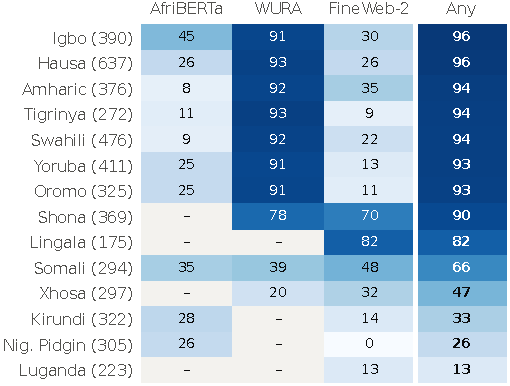
\includegraphics[width=\columnwidth]{figures/contamination.pdf}
\caption{Share of MasakhaNEWS test articles (count in brackets) whose headline, text or URL is in each corpus's training split. ``Any'': in at least one. Dash: the corpus does not cover the language.}
\label{fig:contamination}
\end{figure}

\paragraph{Most test articles are in at least one corpus.} 3,752 of the 4,872 test articles (77\%) are in the training split of at least one audited corpus (Figure~\ref{fig:contamination}; counts in Appendix Table~\ref{tab:counts}). For eight languages the share is 90\% or more. The dev sets look the same (1,875 of 2,429, 77\%).

\paragraph{WURA contains almost entire test sets.} WURA's training split contains 3,116 of the 3,847 test articles in the languages it covers (81\%), and 91--93\% for Amharic, Hausa, Igbo, Oromo, Swahili, Tigrinya and Yoruba, as complete documents with headline, text and URL. The remaining 7--9\% of those test sets are in WURA's eval split: of the 4,827 dev and test articles matched by URL, 9.4\% are there, as expected from a random 90/10 split. WURA's focused crawls of news publishers \citep{oladipo2023wura} reached the same BBC pages that MasakhaNEWS was built from, and nothing in the corpus's construction removed them.

\paragraph{FineWeb-2 and AfriBERTa.} FineWeb-2 contains 28\% of the test articles overall, but 82\% for Lingala and 70\% for Shona, mostly as the original pages. AfriBERTa contains 24\%, mainly through headlines: 891 of 3,803 test headlines (23.4\%) are in its training split, but only 180 articles have half of their 13-grams there.

\paragraph{How headlines leak.} Of the 890 leaked AfriBERTa headlines we could locate, 310 (35\%) form a line of their own, 38 come with a short caption or date, and 542 (61\%) sit inside longer lines: whole BBC pages flattened into one line, with navigation menus (such as the Amharic ``skip to main content'' link) and lists of related stories (Oromo \om{Odeessa kana irratti dabalata}, Pidgin \om{Another thing we de for inside dis tori}). These lines contain many headlines but little article text, so the 13-gram test, which looks for the article body, misses them. Phrase-level matching of short evaluation fields is therefore needed for any benchmark whose inputs or outputs include titles, headlines or summaries.

\paragraph{Little clean data remains.} Only 1,120 of the 4,872 test articles (23\%) are in none of the audited training splits. For nine languages this leaves 15--37 test articles (Appendix Table~\ref{tab:counts}), too few for a reliable estimate of five-way topic accuracy. Five languages keep more: Kirundi, Pidgin and Luganda because WURA does not cover them, and Somali and Xhosa because WURA contains fewer of their articles.

\section{Do Models Remember Contaminated Articles?}
\label{sec:effect}

Overlap shows exposure, not effect \citep{magar2022contamination}. To measure the effect, we need articles the model saw and comparable articles it did not see.

\paragraph{Design.} WURA assigned its documents to train and eval at random, so the benchmark articles it contains were assigned by chance. We compare articles in WURA's training split (\emph{seen}) with articles that are only in WURA's eval split and in no other audited training data (\emph{held out}). Both groups come from the same publishers and time period. We use all 265 held-out dev and test articles in 10 languages and a fixed random sample of up to 150 seen articles per language (1,436). As a balance check, models that were never trained on WURA should score both groups alike; Table~\ref{tab:effect} shows they do.

\paragraph{Models and measure.} We test AfriTeVa~V2 base (428M parameters) and large (1B), T5 models \citep{raffel2020t5} pretrained on WURA, by their pretraining task: 15\% of the tokens are masked in spans of mean length 3 and the model reconstructs them (two fixed masks per article). We test AfriqueQwen3.5-0.8B and -4B-50Langs, continued from Qwen3.5 \citep{qwen2026qwen35} on FineWeb-2, WURA and MADLAD-400, by next-token loss, and also after subtracting the loss of the same model before African-language training (Qwen3.5-0.8B/4B-Base), which removes how hard an article is in itself. Every model reads the first 256 tokens of the headline and text. We report the gap in mean loss between held-out and seen articles, and the AUC: the probability that a seen article has lower loss than a held-out article in the same language (0.5 means no memorization), averaged over languages weighted by held-out articles. $p$-values come from 10,000 permutations of the seen/held-out labels within each language; intervals are 95\% bootstrap intervals.

\begin{table}[t]
\centering
\small
\setlength{\tabcolsep}{2.5pt}
\begin{tabular}{@{}lrrr@{}}
\toprule
Model & Gap & AUC [95\% CI] & $p$ \\
\midrule
\multicolumn{4}{@{}l}{\emph{Trained on WURA}} \\
AfriTeVa V2 base (428M) & 0.3\% & 0.50 [0.46, 0.54] & 0.42 \\
AfriTeVa V2 large (1B) & 1.3\% & 0.51 [0.47, 0.55] & 0.21 \\
AfriqueQwen 0.8B & 3.1\% & 0.55 & 0.005 \\
\quad minus its base & & 0.53 [0.49, 0.56] & 0.04 \\
AfriqueQwen 4B & \textbf{10.0\%} & \textbf{0.64} & \textbf{0.0001} \\
\quad minus its base & & \textbf{0.64 [0.60, 0.67]} & \textbf{0.0001} \\
\midrule
\multicolumn{4}{@{}l}{\emph{Not trained on WURA (balance check)}} \\
Qwen3.5 0.8B base & 0.4\% & 0.51 [0.47, 0.55] & 0.27 \\
Qwen3.5 4B base & 0.3\% & 0.51 [0.47, 0.55] & 0.38 \\
\bottomrule
\end{tabular}
\caption{Memorization of contaminated benchmark articles: 1,436 seen versus 265 held-out articles, assigned by WURA's random split. Gap: how much lower the mean loss is on seen articles. $p = 0.0001$ is the smallest value 10,000 permutations can give.}
\label{tab:effect}
\end{table}

\begin{figure}[t]
\centering
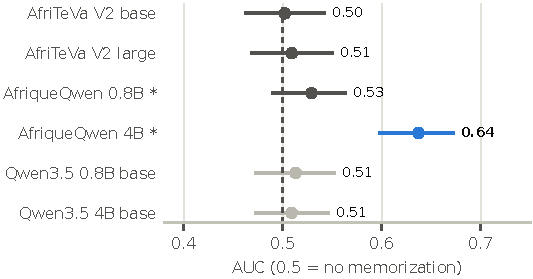
\includegraphics[width=\columnwidth]{figures/memorization.pdf}
\caption{Memorization grows with model size. AUC that a seen article has lower loss than a held-out one, with 95\% bootstrap intervals. *: after subtracting the base model's loss.}
\label{fig:memorization}
\end{figure}

\paragraph{Results.} AfriTeVa~V2 shows no measurable memorization at either size (Table~\ref{tab:effect}): seen and held-out articles are reconstructed equally well (AUC 0.50 and 0.51). Its reported MasakhaNEWS scores are therefore unlikely to be inflated by memorized test articles, even though most of them were in its training data. AfriqueQwen behaves differently. At 0.8B parameters seen articles have 3.1\% lower loss (AUC 0.55, $p = 0.005$); after removing article difficulty the effect is weak (AUC 0.53, $p = 0.04$, interval touching 0.5). At 4B the gap is 10.0\% and the AUC 0.64, with or without the correction (Figure~\ref{fig:memorization}). The base models before African-language training show no difference between the groups, so the effect comes from training on WURA, not from how the groups were formed.

\begin{figure}[t]
\centering
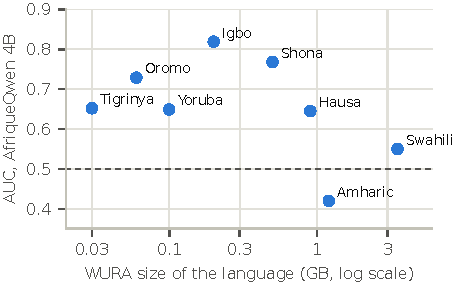
\includegraphics[width=\columnwidth]{figures/by_language.pdf}
\caption{Memorization by language: AfriqueQwen 4B, after subtracting its base model's loss, against the size of the language in WURA. Languages with at least 15 held-out articles.}
\label{fig:lang}
\end{figure}

\paragraph{Where memorization happens.} The 4B effect is uneven across languages (Figure~\ref{fig:lang}): AUC 0.82 for Igbo, 0.77 for Shona and 0.73 for Oromo, but 0.55 for Swahili and 0.42 for Amharic, the two languages with the most WURA data. AfriqueLLM's training recipe caps high-resource languages and upsamples lower-resource ones for up to five epochs \citep{yu2026afriquellm,chung2023unimax}, and repeated text is memorized more \citep{carlini2023quantifying,kandpal2022dedup}. The rank correlation between WURA size and AUC is negative ($\rho = -0.60$) but, with eight languages, not significant ($p = 0.12$); we report it as consistent with repetition-driven memorization rather than as proof.

\section{Discussion}

\paragraph{Exposure is nearly universal; effect depends on the model.} Because MasakhaNEWS was built from public news pages, any corpus that crawls those publishers will contain it, and three widely used corpora do. Whether this distorts evaluation depends on the model. A T5 model trained on a 30\,GB corpus shows no detectable memorization; a 4B decoder whose recipe repeats low-resource text does, and more than its 0.8B sibling. As African language models grow and their low-resource data is repeated to balance languages, the same benchmark will increasingly overstate them, and most for the languages with the least data.

\paragraph{Recommendations.} \emph{Benchmark builders} should check new test sets against the major public corpora before release, and prefer sources that are not crawled or publish after corpus cut-off dates. \emph{Corpus builders} should remove known evaluation sets, including headlines and other short fields, and document it; WURA's URL-based deduplication would make this simple. \emph{Model developers} should report overlap with every benchmark they use and evaluate on clean subsets. For MasakhaNEWS, the clean subsets are too small for nine languages, so new test articles are needed.

\section*{Limitations}
\label{sec:limits}

We audited three corpora; MADLAD-400 and other web corpora were not checked, so the clean subsets are clean only with respect to these three. URL matching relies on recorded URLs, and text matching on exact tokens; paraphrased or translated copies are not detected. The memorization study measures loss, not downstream task accuracy, and topic labels are not part of the leaked text; it shows that models can tell seen from held-out articles, not by how much reported scores are inflated. The held-out groups are small (15--49 articles in each of the eight languages we report individually, and 1 and 5 for Somali and Xhosa), so per-language estimates are uncertain. The study assumes WURA's train/eval assignment is random, which the 9.4\% eval share and the balance check support but cannot prove. Somali and Xhosa have few held-out articles, and Xhosa's test set comes from a different source (\om{Isolezwe lesiXhosa}) than most others. We did not audit other BBC-based benchmarks such as XL-Sum, which WURA's authors also evaluate on and which deserve the same check.

\section*{Ethics Statement}

The audit uses only public datasets and corpora under their licenses (MasakhaNEWS AFL-3.0, AfriBERTa corpus Apache-2.0, WURA Apache-2.0, FineWeb-2 ODC-By). We release per-article flags and indices into the official benchmark files, not benchmark or corpus text. Contamination of this kind is a consequence of how scarce African-language text is and of reasonable choices by dataset builders; our aim is to make evaluation more reliable, not to fault prior work, whose authors made their data and models openly available and thereby made this audit possible.

\section*{Acknowledgments}

This work was carried out with substantial assistance from an AI assistant (Claude, by Anthropic), which wrote much of the code and a first draft of the text under the author's direction. The author chose the research question, directed the experiments, reviewed the results and takes full responsibility for the content.

\bibliography{references}

\appendix

\section{Counts and Clean Subsets}

\begin{table}[h]
\centering
\small
\setlength{\tabcolsep}{2.5pt}
\begin{tabular}{@{}lrrrrrr@{}}
\toprule
Language & Test & AfriB. & WURA & FW-2 & Any & Clean \\
\midrule
Amharic & 376 & 31 & 345 & 132 & 354 & 22 \\
Hausa & 637 & 165 & 592 & 165 & 612 & 25 \\
Igbo & 390 & 174 & 356 & 117 & 375 & 15 \\
Kirundi & 322 & 89 & -- & 45 & 107 & 215 \\
Lingala & 175 & -- & -- & 143 & 143 & 32 \\
Luganda & 223 & -- & -- & 30 & 30 & 193 \\
Nig. Pidgin & 305 & 78 & -- & 0 & 78 & 227 \\
Oromo & 325 & 82 & 296 & 35 & 303 & 22 \\
Shona & 369 & -- & 287 & 259 & 332 & 37 \\
Somali & 294 & 102 & 114 & 141 & 193 & 101 \\
Swahili & 476 & 45 & 440 & 103 & 446 & 30 \\
Tigrinya & 272 & 29 & 254 & 24 & 256 & 16 \\
Xhosa & 297 & -- & 59 & 96 & 139 & 158 \\
Yoruba & 411 & 104 & 373 & 54 & 384 & 27 \\
\midrule
Total & 4872 & 899 & 3116 & 1344 & 3752 & 1120 \\
\bottomrule
\end{tabular}
\caption{MasakhaNEWS test articles in each corpus's training split, and articles in none of them (clean). Dash: corpus does not cover the language.}
\label{tab:counts}
\end{table}

\section{Reproducibility}

All results come from numbered scripts in the \texttt{audit/} folder of the public repository (\url{https://github.com/HabtamuFeyera/afaan-oromoo-llm}), run on one Apple M1 Max laptop with 64\,GB of memory: downloads (\texttt{01}), overlap (\texttt{02}; under 30 minutes for all corpora), summary (\texttt{03}), groups, scoring and statistics for the memorization study (\texttt{04}--\texttt{06}; 4--29 minutes per model), release files (\texttt{07}), leak mechanism (\texttt{08}) and figures (\texttt{09}). One detail matters for anyone reusing AfriTeVa~V2: the model was trained with the last SentencePiece ids (149999, 149998, \dots) as sentinel tokens, not the 100 extra ids that the Hugging Face T5 tokenizer appends. With the latter, its span-corruption loss is above chance (about 12 nats per token); with the former it is 0.2--0.7 on ordinary text.

\end{document}
